\documentclass{article}
\usepackage{graphicx}

\begin{document}

%test results and analysis
\section{Measurements}
In this section below, the test results of the new algorithm can be seen. The SAT problem is NP-complete, which means most of the modern algorithms' computational cost are close to exponential. But our method provides $n^{2}$ computational cost.

\subsection{Test results}
During testing we ran our algorithm and one of our most efficient on SAT problems. We tried the algorithms on logical formulas, that contains 1 to 4 logical variables. The methods got the same formulas, problems. The results of the executions are shown the diagrams below.

On the diagrams the blue dots represents our algorithm max and min computational costs for each amounts of logical variables. The red dots represents the concurrent algorithms minimal computational cost. The blue line shows the average costs of our algorithm, the read one belongs to the best concurrent algorithms. For instance the SAT-3 problem solved in only 9 steps.

\begin{figure}[h]
    \centering
    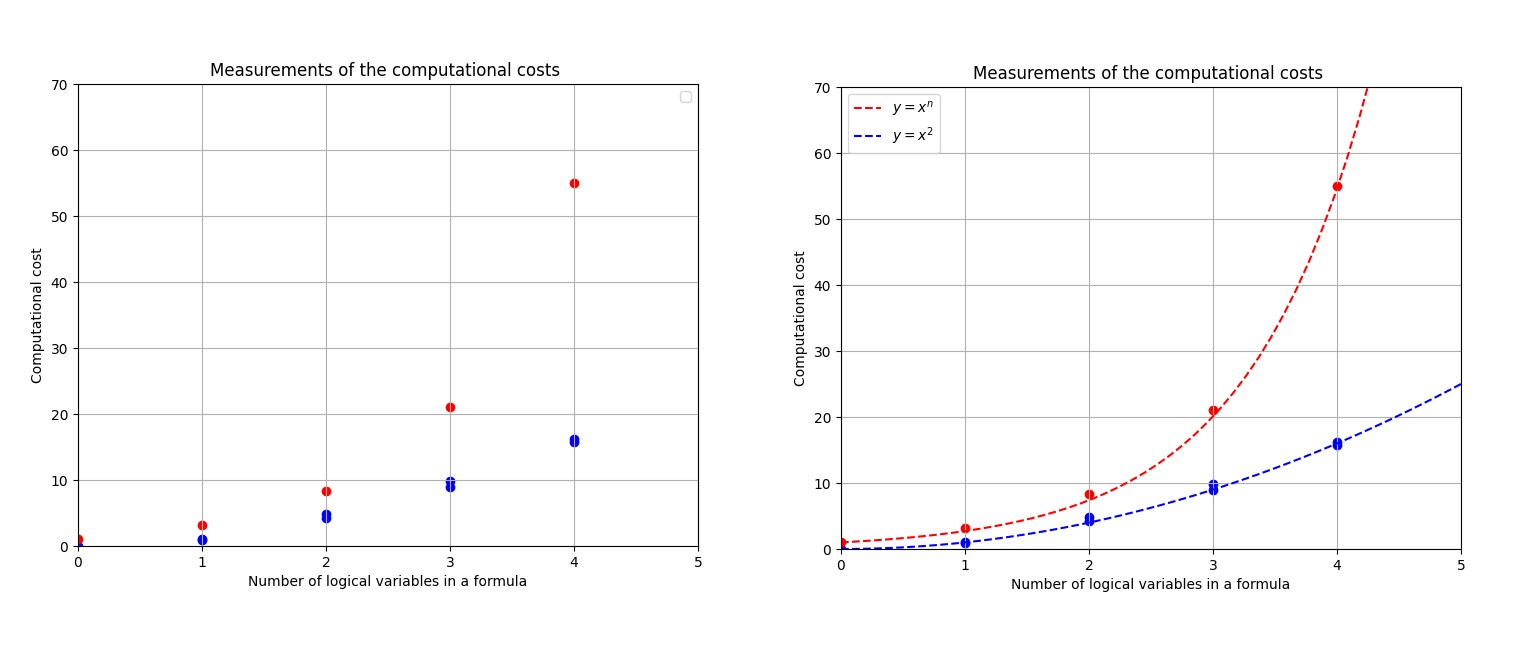
\includegraphics[width=1\linewidth]{img/measurements.png}
\end{figure}

\subsection{Analysis}
It seems, that due to the dissimilar average computational costs, major magnitude differences formed. The new method for SAT solution, provides $n^{2}$ computational cost, because of the advanced heuristic model.This cause a great advantage against the concurrent algorithms.

\end{document}
